\STAIF{} is an automated instrumentation framework that combines
distributed tracing and control logic based on the principles.  It is
deployed alongside running distributed applications.  In normal
operation, \STAIF{} operates identically to existing distributed
tracing, generating traces using tracepoints that developers wish to
have always on.  These tracepoints may be ones developers have found
useful in the past or ones used for use cases other than performance
diagnosis, such as correctness.  When new performance problems occur,
developers can use \STAIF{} to automatically enrich traces with the
additional tracepoints needed to localize them.

\STAIF{} localizes problems due to slow code or those with
unpredictable performance (high variance).  Such unpredictability may
emanate from areas of the application itself, third-party code the
application uses, or from areas of the application that could benefit
from additional tracing instrumentation. \STAIF{}
also explores whether key/value pairs exposed in tracepoints explain
high variance.  It allows developers to specify important keys that
they suspect will explain variance and bin ranges for them.  \STAIF{}
will augment tracepoint names with these keys if they explain
variance.  It will surface other keys whose values explain variance in
its output.

Like manual dynamic-instrumentation
approaches~\cite{Erlingsson:2011wy, Mace:2015uh}, \STAIF{} frees
developers from the tussle between generality and overhead.  Unlike
manual approaches, it also frees them from having to search the space
of tracepoint choices to enable additional ones.  When enabling
instrumentation, \STAIF{} works in a continuous cycle.  At each
iteration, it uses the principles to hypothesize (guess) which
tracepoints should be enabled next within a high variance or slow area
of the application.  It uses the results of previous hypotheses to
guide future ones.  It uses a novel data structure, called
the \textit{hypothesis forest}, to explain the results of its
hypotheses to developers.  \STAIF{}'s analyses are most useful for
on-path problems.  It also provides value for off-path problems by
identifying the critical-path areas most affected by them.

%
\mert{
  1. Removed last paragraph here (of discussions)
}
% The rest of this section describes \STAIF{} in more detail.  
% Our discussions are agnostic to whether tracepoints are enabled or
% disabled using dynamic instrumentation~\cite{Erlingsson:2011wy,
% Cantrill:2004dtrace, Mace:2015uh} or by modifying existing tracing
% infrastructures' tracepoints to execute conditional checks before
% emitting tracepoint records.  We assume tracepoints are uniquely
% addressable.  Some methods for addressing them include using: their
% names (as done for Linux kernel logs); hashes of their names and their
% keys (if names are not unique); an external registry that assigns
% addresses to tracepoints.  We assume unique names from now on.

\subsection{Design}
Figure~\ref{fig:staif_design} shows \STAIF{}'s design, which builds
upon existing distributed tracing.  It consists of a
control plane and an instrumentation plane.  Components in the
\textit{control plane} implement the control logic whereas
those in the \textit{instrumentation plane} implement the control
logic's hypotheses or provide custom information about the
application.

\STAIF{} works in a continuous loop, which is shown in \textit{red}
in the figure.  At each iteration, \STAIF{}'s instrumentation-plane
components gather new critical-path traces (
\includegraphics[scale=0.5, trim=-0 0.3cm 0 0]{figures/marked_A.pdf} in the figure).
The control-plane components examine them to identify hypotheses of
which tracepoints should be enabled next and which key/value pairs
additionally explain high variance (
\includegraphics[scale=0.5, trim=-0 0.3cm 0 0]{figures/marked_B.pdf}).  Hypotheses are sent to
the instrumentation plane components (
\includegraphics[scale=0.5, trim=-0 0.3cm 0 0]{figures/marked_C.pdf}), which enable the
relevant tracepoints and the cycle repeats. \STAIF{}
pauses its explorations if any of the tracing agents' queues are
congested.  This prevents cases in which \STAIF{} does not observe the
effects of new hypotheses because tracepoints records were dropped.

\begin{figure}[tb]
    \centering
    % \vspace{-0.1cm}
    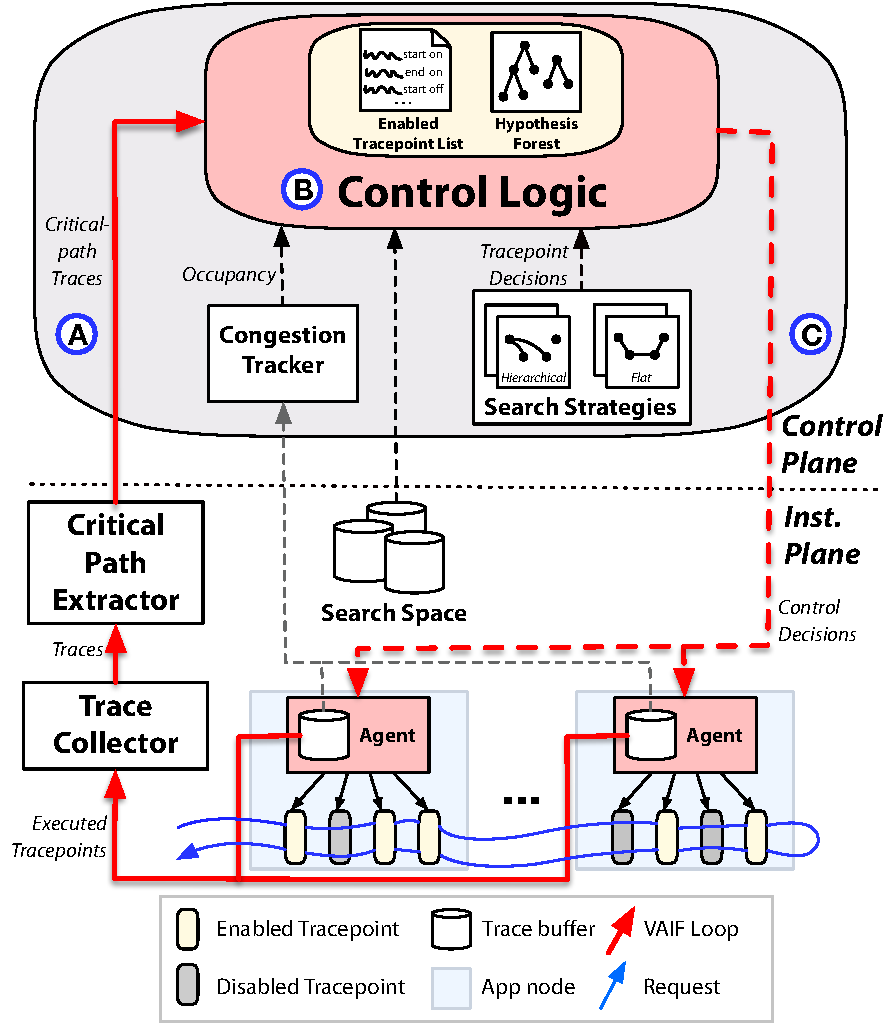
\includegraphics[width=\columnwidth]{figures/fig_staif_design.pdf}
    % \vspace{-0.8cm}
  
    \caption{\STAIF{} design. The thick red line shows \STAIF{}'s
      continuous loop.  Solid lines are traces/tracepoints and dashed
      lines are control signals.  A generic distributed application
      instrumented with tracing is shown in the instrumentation plane.}
    
    \label{fig:staif_design}
     \vspace{-0.2in}
  \end{figure}


  \subsubsection{Components}
  \label{sec:design:components}
%   \hfill\\
  \noindent\textbf{Control plane} The control plane consists of the
  control logic, two search strategies for deciding which tracepoints to
  enable in high-variance or slow areas, and a congestion tracker that
  periodically receives queue occupancies from tracing agents.  The
  search strategies are designed to be generically applicable to many
  distributed applications.  The congestion tracker informs the control
  logic when any tracing agents' queues are in danger of being
  congested, which we define as over 50\% occupancy.  We use this
  conservative definition because \STAIF{} does not know how many times
  tracepoints will execute once enabled.  The control plane also
  maintains important state: a global list of tracepoints that have been
  enabled by \STAIF{}{} and the hypothesis forest.
  
  \STAIF{}'s control-plane components are modular and intended to
  be used with different distributed applications and/or
  tracing infrastructures without modifications.
  
  \noindent\textbf{Instrumentation plane} The instrumentation plane
  consists of an application instrumented with tracing, a critical-path
  extractor that extracts critical-path portions from traces and sends
  them to \STAIF{}'s control-plane components, and a search space that
  describes the application's tracepoints.  The critical-path extractor
  works by identifying the highest-latency trace path from the
  tracepoint indicating request reply to that indicating request start.
  Concurrency and synchronization may result in multiple paths for a
  single trace, each with different latencies.  The search space names
  all of the tracepoints in the distributed application, including the
  keys that will be used in grouping.  It also lists
  concurrency/synchronization tracepoint names as these must be enabled
  for critical-path extraction.
  
  Legacy instrumentation-plane components require modifications to be
  used with \STAIF{}.  First, the tracing
  infrastructure's libraries must allow tracepoints to be selectively
  enabled or disabled during runtime.  They must also let developers
  specify which tracepoints should be considered always on. Second,
  tracing agents co-located with processes must report queue lengths and
  receive updates about which tracepoints to enable or disable. Third,
  tracing infrastructures must preserve happens-before relationships
  between tracepoint records to allow critical paths to be
  extracted. This can be done by exposing APIs to capture them directly
  (as done by X-Trace~\cite{Fonseca:2010vn, Mace:ui},
  Canopy~\cite{Kaldor:2017gp}, and Stardust~\cite{Sambasivan:2011vw}) or
  by learning them over a large number of traces (as done for traces
  that preserve only hierarchical caller/callee relationships, such as
  Dapper~\cite{Mann:2011vf} and Artillery~\cite{Chow:2014ts}).
  
  \vspace{-0.05in}
  \subsubsection{Usage}
  \label{sec:design:init}
  \hfill\\
  \noindent\textbf{Starting \STAIF{}'s exploration} \STAIF{} takes 
  two inputs to start its explorations.  The first is the application
  search space.  The second is a list of tracepoints corresponding to start
  of execution of request types (or endpoints) that are experiencing
  problems.  (We assume tracepoints that name the corresponding replies
  can be programmatically derived otherwise, they would need to be
  provided as well.)
  
  \STAIF{} also takes as input two optional parameters.  
  The first is a threshold for identifying groups of critical-path
  traces that exhibit high variance, specified as a coefficient of
  variation (CV or $\sigma/\mu$).  We use CV for this unpredictability
  condition because it is a unitless measure that reflects the intuition
  that groups with high response-time spread compared to their mean are
  more unpredictable than those with low spread.  The second is a
  threshold for identifying groups as consistently slow (CS). It is
  specified as a percentile of the relevant request type's response-time
  distribution.  \STAIF{} considers any group of traces that show either
  CV or mean latency greater than these thresholds as potential
  problems.  Default values of : CV threshold = 10\%, CS threshold =
  95\% are used if these optional parameters are not specified.
  
  \noindent\textbf{\STAIF{}'s output and how to use it}
  \STAIF{} outputs new traces whose critical paths
  are enriched with the additional tracepoints needed to localize
  problems.  Developers can query the hypothesis forest to identify why
  tracepoints observed in a given trace were enabled.  For example, for
  a given trace, the forest might show that enabling a tracepoint around
  a cache differentiated critical paths and generated two new groups,
  increasing predictability (lower CV) for one group and isolating
  unpredictability (increasing CV) for the other group.  Developers can
  also examine the hypothesis forest directly to identify groups of
  requests with high response-time variation or groups that are
  consistently slow.
  
  \noindent\textbf{Shutting down \STAIF{}} Developers can shut down \STAIF{}
  after they have diagnosed the problem at hand.  Before
  terminating, \STAIF{} will disable all of the additional tracepoints
  it enabled.

  \subsection{Hypothesis forest}
\label{sec:design:control_logic}

At each cycle, \staif{}'s control logic explores hypotheses of which
tracepoints should be enabled to localize problems.  Hypotheses
themselves are of the form ``differentiating traces by whether they
include or a lack a newly-enabled tracepoint helps localize the
problem.''  Localization amounts to 1) differentiating groups of
identical critical-path traces with high variance, 2) isolating
high-variance application areas within groups, or 3) isolating
application areas that lead to consistently-slow performance.  To
explain its decisions, it maintains a history of its hypotheses and
their outcomes in the hypothesis forest.  

% We describe the hypothesis
% forest first, then how the control logic explores hypotheses and
% constructs the forest.

% \subsubsection{Hypothesis forest}

{
\begin{figure}[tb]
  \centering
 
  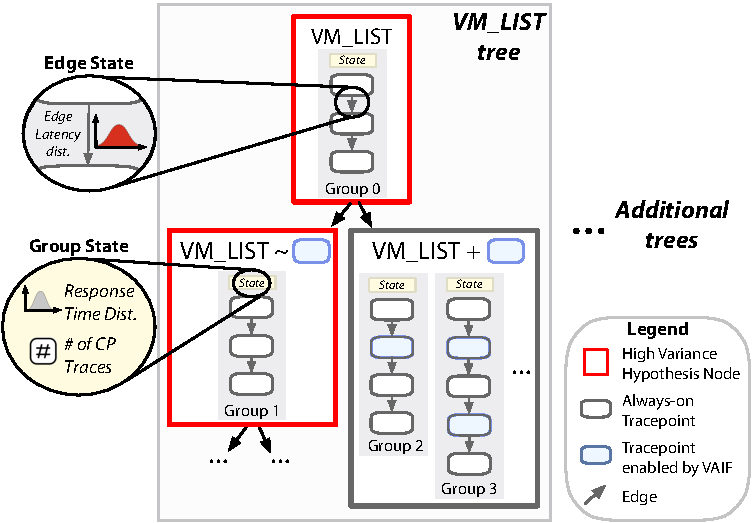
\includegraphics[width=\columnwidth]{figures/hypo.pdf}
 
  \caption{\STAIF{}'s hypothesis forest. This figure shows a \textsc{VM\_LIST} tree from the forest}
  \label{fig:hyp_tree}
   
\end{figure}
}

Figure~\ref{fig:hyp_tree} shows an example hypothesis forest.  Each
tree in the forest encodes hypotheses made on behalf of a different
request type or endpoint that \STAIF{} is initialized with (e.g.,
OpenStack's \textsc{VM\_LIST} in the figure).  This reflects the
intuition that request type is a basic predictor of performance and
that different request types may experience different problems
that benefit from different tracepoints.



Nodes of hypothesis trees (hypothesis nodes) contain pointers to the
results of applying hypotheses. Hypotheses result in two
nodes, one for traces that include the enabled tracepoint and the other
for ones in which it is absent.  Each node includes a field that
names the hypothesis tracepoint and whether it should be present or
absent from traces (e.g., $+$
\includegraphics[scale=0.7, trim=-0 0.1cm 0 0]{figures/blue_bubble.pdf} or $\sim$ 
\includegraphics[scale=0.7, trim=-0 0.1cm 0 0]{figures/blue_bubble.pdf} in the
figure).  The root node of each tree shows results for traces that
include the request-type start tracepoint.

Results are: 1) groups of identical critical-path
traces that either include or exclude the tracepoint and 2) any keys
in included tracepoints that explain variance.  Groups store important
performance information needed for \STAIF{}'s analyses--a
representative trace, response-time distributions of requests assigned
to them, trace edge-latency distributions, and the number of requests
assigned to each group.  Tracepoints enabled by \STAIF{} on behalf of
other paths or trees are removed from traces before grouping.  Such
processing allows \STAIF{} to measure the effects of each hypothesis
independently w/o interference from other hypotheses.  Always-on
tracepoints are not removed as \STAIF{} does not make hypotheses about
them.

\mert{Removed control logic pseudo code and walkthrough. We already talked about control logic so far in high level.}

\subsection{Search space \& search strategies}
\label{sec:design:search_strategies}

\noindent\textbf{Search space} The search space contains: 1) potential
critical paths in requests' workflows when all tracepoints are
enabled; 2) tracepoints that demarcate concurrency or
synchronization; 3) keys within tracepoints that should be
incorporated in grouping and bin ranges for them. % (needed for $search.key\_value()$).   %MERT: there is no search.augment
% All tracepoints are labeled with whether they are always on. % MERT: do we really need to say this
  % (which we assume is a key/value pair).  
Search strategies use the search space to suggest the next tracepoint to
enable between high-variance or -latency trace edges.  %(i.e., $search.find()$)
This requires \textit{matching} the group
critical-path trace representative against potential critical paths in
the search space to determine which path it is most likely to be.

\textit{Potential critical paths:} These are learned by
running exhaustive workloads against the application with all
tracepoints enabled. For traces with multiple
concurrent branches, each unique path within them is stored separately as a
potential critical path. We expect potential critical paths will be
learned as part of organizations' code or coverage tests.  These tests
can be run when deploying an application or updating it.  
\STAIF{} will still provide value if the paths stored in the
search space are incomplete.

\textit{Developer-specified keys and bin ranges:} These are stored as
key name, tracepoint to which they belong, and a set
of bin ranges.  We expect developers will specify only a few select
keys (e.g., ones that correspond to request sizes or ones that
indicate queue lengths for a highly-contended resource.)

\textit{Concurrency / synchronization points:}
These are identified automatically as fan-out and fan-in points in
learned paths.

\textit{Matching to potential critical paths:} For a given group, we transform
its representative trace into a regular expression.  
For example, the trace ``\texttt{A->B->C}'' is
transformed into ``\texttt{.*A.*B.*C.*}''.  The
expression is applied to all potential critical paths to identify
potential matches.  
% MERT: following is removed for trimming
% False matches that include always-on tracepoints that are not contained the group representative trace are discarded.
We choose among multiple matching potential critical paths randomly
\textcolor{red}{(weighted by frequency of their occurrence during learning)}.


%strategy iterates the paths in the search space concurrently. For any
%node (tracepoint) in the group representative, it iterates the
%potential critical paths until an identical node is found. More
%formally, the group representative path ``\texttt{ABC}'' is
%transformed into the regular expression ``\texttt{.*A.*B.*C.*}''.  We
%choose among multiple matching potential critical paths randomly
%weighted by frequency of their occurrence during learning.

\noindent\textbf{Search strategies} The two search strategies either
use the hierarchical or happens-before edges in traces.

% \raja{This is too simple...we did something about areas between spans.}

\textit{Hierarchical search}: This strategy
uses hierarchical edges (called spans in
OpenTelemetry~\cite{opentelemetry}).  Given a pair of tracepoints
that denote a hierarchical level (a span), this strategy determines
which pair of tracepoints (subspan) to enable next.  In the case where
there are multiple subspans, we use binary search to pick the middle
one.

\textit{Flat search:} This strategy uses only
the happens-before relationships.  Given a pair of tracepoints, this
picks a tracepoint that occurs between them.
Tracepoints are ordered by happens-before
relationships and binary search is used to pick among them.


\mert{
  1) Removed Limitations. 2)
}
